\section{链初值的影响}
\label{sec:mcerr-initial}

现在设转移是精确的。第~\ref{chap:sample-generation}章用转移核$K(x,A)$描述链：当前状态为$x$时，下一状态落入$A$的概率为$K(x,A)$。若
\[
 \int_{\mathcal{X}}K(x,A)\,\pi(\mathrm{d}x)=\pi(A)\qquad\text{对每个事件}A ,
\]
就称$\pi$是不变分布。链从$X^{(0)}$出发，依次生成$X^{(1)},X^{(2)},\dots$，用
\begin{equation}
 \hat{I}_N=\frac1N\sum_{t=1}^{N}f\bigl(X^{(t)}\bigr)
 \label{eq:mcerr-chain-average}
\end{equation}
估计$I$。这一节研究链从哪里出发怎样影响这个平均的偏差。

\paragraph{从目标分布出发}
若$X^{(0)}\sim\pi$，由不变性，$X^{(1)}$的分布是
\[
 \mathbb{P}(X^{(1)}\in A)=\int K(x,A)\,\pi(\mathrm{d}x)=\pi(A) ,
\]
依次类推，每个$X^{(t)}$都服从$\pi$。由第~\ref{sec:mcerr-estimator}节，偏差只看各项的分布，所以$\hat{I}_N$无偏，尽管各项高度相关。这样的链称为平稳的：任意时刻的状态都服从$\pi$。

\paragraph{从一般初值出发}
实际中能精确从$\pi$出发，往往就不需要链了。设$X^{(0)}\sim\mu$。记$K^{t}(x,\cdot)$为从$x$出发$t$步后状态的分布，则$X^{(t)}$的分布是$\mu K^{t}=\int\mu(\mathrm{d}x)\,K^{t}(x,\cdot)$，一般不等于$\pi$。设各项可积，偏差为
\begin{equation}
 b_N=\frac1N\sum_{t=1}^{N}\Bigl(\mathbb{E}_{\mu K^{t}}[f]-I\Bigr) .
 \label{eq:mcerr-initial-bias}
\end{equation}
偏差的大小取决于边缘分布$\mu K^{t}$趋近$\pi$的快慢。

\paragraph{一条可以算到底的链}
下面这条链贯穿本章后半部分。取$\pi=\mathcal{N}(0,1)$，$\lvert\rho\rvert<1$，令
\begin{equation}
 X^{(t+1)}=\rho X^{(t)}+\sqrt{1-\rho^{2}}\,\xi^{(t+1)} ,
 \label{eq:mcerr-ar1}
\end{equation}
其中$\xi^{(t)}$独立且服从$\mathcal{N}(0,1)$，与$X^{(0)}$独立。若$X^{(t)}\sim\mathcal{N}(0,1)$，则$X^{(t+1)}$服从均值为$0$、方差为$\rho^{2}+(1-\rho^{2})=1$的高斯分布，所以$\pi$是不变分布。$\rho$越接近$1$，每步保留的旧状态越多，链移动越慢。

从$X^{(0)}=x_0$出发，展开递推，
\[
 X^{(t)}=\rho^{t}x_0+\sqrt{1-\rho^{2}}\sum_{j=1}^{t}\rho^{t-j}\xi^{(j)} .
\]
后一项是独立高斯变量的线性组合，方差为$(1-\rho^{2})\sum_{j=0}^{t-1}\rho^{2j}=1-\rho^{2t}$，所以
\begin{equation}
 K^{t}(x_0,\cdot)=\mathcal{N}\bigl(\rho^{t}x_0,\ 1-\rho^{2t}\bigr) .
 \label{eq:mcerr-ar1-marginal}
\end{equation}
均值以几何速度$\rho^{t}$忘掉初值。对$f(x)=x$，$I=0$，由式~\eqref{eq:mcerr-initial-bias}，偏差为几何级数之和：
\[
 b_N=\frac{x_0}{N}\sum_{t=1}^{N}\rho^{t}=\frac{x_0\,\rho\,(1-\rho^{N})}{N(1-\rho)} .
\]

取$\rho=0.9$，$x_0=10$。偏差约为$90/N$：
\[
 b_{100}=0.900,\qquad b_{1000}=0.0900 .
\]
第~\ref{sec:mcerr-long-run}小节会算出平稳时这条链平均的标准差约为$\sqrt{19/N}$，$N=100$时为$0.436$，比偏差还小。偏差按$1/N$缩小，标准差按$1/\sqrt{N}$缩小，所以记录足够长时初值的影响终将被波动淹没，但在中等长度上它可以是误差的主要部分。图~\ref{fig:mcerr-burnin}(a)是$20$条从$10$出发的路径，它们沿着$0.9^{t}\times10$向$0$靠拢，大约$40$步以后才混入平稳的波动带。

\paragraph{舍弃初始一段}
常用的办法是先运行$b$步不记录，再平均接下来的$N$个状态，被舍弃的这一段称为\term{预烧期}（burn-in period）。对上面的链，平均$X^{(b+1)},\dots,X^{(b+N)}$的偏差是
\[
 \frac{x_0\,\rho^{b+1}(1-\rho^{N})}{N(1-\rho)} .
\]
$N=100$时，$b=20$把偏差从$0.900$降到$0.109$，$b=50$降到$0.0046$，如图~\ref{fig:mcerr-burnin}(b)。

\begin{BookInlineFigure}
 \centering
 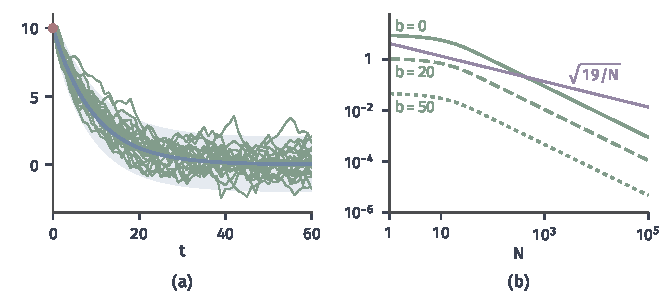
\includegraphics[width=112mm]{figures/07-probability/08-sampling-and-integration/matplotlib/mcerr-burnin/figure.pdf}
 \caption{链~\eqref{eq:mcerr-ar1}在$\rho=0.9$时从$x_0=10$（红点）出发。(a)$20$条路径（绿线，种子$3122$），蓝线为边缘均值$0.9^{t}x_0$，浅蓝带为边缘均值加减两倍边缘标准差；(b)舍弃前$b$步后平均$N$步的偏差精确值（绿色实线、虚线、点线分别为$b=0,20,50$），紫线为平稳时的标准差$\sqrt{19/N}$，双对数坐标。}
 \label{fig:mcerr-burnin}
\end{BookInlineFigure}

预烧期之所以有效，是因为这里知道边缘分布以$\rho^{t}$的速度靠近$\pi$。一般地，若对有界的$f$已知$d_{\mathrm{TV}}(\mu K^{t},\pi)\leq Cr^{t}$，$0<r<1$，由式~\eqref{eq:mcerr-tv-bound}与式~\eqref{eq:mcerr-initial-bias}，舍弃$b$步后
\begin{equation}
 \lvert b_N\rvert\leq\frac{\operatorname{osc}(f)}{N}\sum_{t=b+1}^{b+N}Cr^{t}\leq\frac{\operatorname{osc}(f)\,C\,r^{b+1}}{N(1-r)} .
 \label{eq:mcerr-burnin-bound}
\end{equation}
没有这类收敛控制，预烧期就没有依据。最极端的例子是始终停在原地的转移$K(x,\cdot)=\delta_{x}$：每个分布都是它的不变分布，但从$x_0$出发的链永远停在$x_0$，舍弃多少步都不改变$\hat{I}_N=f(x_0)$。第~\ref{sec:mcerr-diagnostics}小节还会看到更隐蔽的情形：链在一个局部区域内看起来已经平稳，却始终没有到达目标的另一部分。

即使有收敛控制，舍弃之后剩下的样本也不是精确平稳的。在式~\eqref{eq:mcerr-ar1-marginal}中，任何有限的$t$都有$1-\rho^{2t}<1$，$K^{t}(x_0,\cdot)$从来不等于$\pi$。预烧期只是把偏差压到可以忽略的量级，这个量级需要由式~\eqref{eq:mcerr-burnin-bound}这样的估计给出。

\paragraph{无界被积函数}
式~\eqref{eq:mcerr-burnin-bound}要求$f$有界。对无界的$f$，即使$\mu K^{t}$收敛到$\pi$，期望也未必收敛。第~\ref{chap:random-variable-convergence}章与第~\ref{chap:weak-convergence-of-distributions}章说明，分布收敛之外还需要$f(X^{(t)})$一致可积，才能保证$\mathbb{E}[f(X^{(t)})]\to\mathbb{E}_{\pi}[f]$。

仍用链~\eqref{eq:mcerr-ar1}，但让$X^{(0)}$服从二阶矩无穷的分布，例如标准Cauchy分布，取$f(x)=x^{2}$。$X^{(t)}=\rho^{t}X^{(0)}+G_t$，其中$G_t$是与$X^{(0)}$独立的高斯变量。给定$G_t$时，$\rho^{t}X^{(0)}+G_t$的二阶矩为无穷，所以对每个$t$，
\[
 \mathbb{E}\bigl[(X^{(t)})^{2}\bigr]=\infty .
\]
另一方面，$\rho^{t}X^{(0)}\to0$依概率成立，由Slutsky定理，$X^{(t)}$依分布收敛到$\mathcal{N}(0,1)$。于是对每个$N$和每个预烧期长度，$\mathbb{E}[\hat{I}_N]=\infty$，偏差没有意义，舍弃初始段也无济于事。初值的尾部经过任意有限步都没有被完全忘掉，正是这种残留破坏了一致可积性。
